\chapter{State of the Art and Technological Choices}

\section*{Introduction}
Selecting technologies for Qatra required more than assembling popular frameworks. Each choice had to support domain modularity, secure web interaction, reliable persistence, asynchronous coordination, and observable deployment. This chapter positions the selected stack against reasonable alternatives.

\section{Digital Blood-Donation Platforms}
A modern blood-donation platform combines three categories of capability. The first is donor engagement: registration, eligibility guidance, location, appointment booking, reminders, and donation history. The second is center operations: capacity, staff tasks, screening, completion, and reports. The third is urgent coordination: emergency creation, compatibility filtering, geographical matching, notification, acceptance, and resolution.

These capabilities share data but have different operational rhythms. Appointment planning is predictable; emergency matching is time-sensitive and bursty. Administrative reporting is read-oriented; screening and emergency response change sensitive state. Architecture must reflect those differences while preserving a coherent user journey.

\section{Architectural Style}
\subsection{Monolith and Microservices}
A modular monolith offers simple deployment and local transactions. It is often appropriate for an early product. Microservices provide stronger deployment and scaling boundaries but introduce distributed communication, observability, and consistency costs~\cite{microservices}. Qatra adopts a pragmatic microservices-oriented structure: a principal donation service contains closely related domain modules, while notification responsibilities are separated. This avoids premature fragmentation into many small services while giving asynchronous delivery a distinct operational boundary.

\begin{table}[H]
\centering\small
\begin{tabularx}{\textwidth}{|P{3.2cm}|Y|Y|Y|}
\hline
\rowcolor{tableheader}\textbf{Criterion} & \textbf{Layered monolith} & \textbf{Fine-grained microservices} & \textbf{Qatra choice}\\ \hline
Deployment simplicity & High & Low & Moderate: two backend services\\ \hline
Local consistency & Strong & Requires coordination & Domain writes remain local where possible\\ \hline
Independent scaling & Limited & High & Notification processing can evolve separately\\ \hline
Operational complexity & Low & High & Controlled through containers and observability\\ \hline
Domain modularity & Depends on discipline & Enforced by boundaries & Hexagonal modules inside the donation service\\ \hline
\end{tabularx}
\caption{Architectural style comparison}
\label{tab:architecture-comparison}
\end{table}

\subsection{Hexagonal Organization}
The donation service organizes many features around domain models, inbound ports, outbound ports, application services, and infrastructure adapters. This reflects hexagonal architecture: business rules depend on abstractions, while persistence and web concerns implement external adapters~\cite{hexagonal}. The benefit is visible in modules such as appointment, center, donor, emergency, and analytics, where domain vocabulary is not reduced to controller or database terminology.

\section{Event-Driven Communication}
Synchronous HTTP is appropriate when a caller needs an immediate response. Notification delivery is different: once a domain event is accepted, email or real-time delivery may take longer or temporarily fail. Kafka supports durable asynchronous exchange and decouples the producer's transaction from downstream processing~\cite{kafka}. The trade-off is eventual consistency and the need for retry, idempotency, correlation, and monitoring.

Qatra uses Kafka in the infrastructure and service configuration as the event backbone between donation-oriented actions and notification processing. The design chapter explains how this boundary is represented without claiming stronger delivery guarantees than the code and configuration demonstrate.

\section{Backend Framework: Java and Spring Boot}
Java 21 provides a current long-term-support runtime with a mature ecosystem. Spring Boot supplies web, validation, security, persistence, actuator, mail, WebSocket, and testing integration~\cite{spring}. The project's Maven descriptors target Java 21 and Spring Boot 4.0.6.

Alternatives such as Node.js or .NET could support the same domain. Spring Boot was retained because the project benefits from typed domain models, mature JPA integration, declarative validation, filter-based security, and consistent operational endpoints. Its main costs are framework complexity and a larger runtime footprint than minimal services.

\section{Frontend Framework: Angular}
Angular provides a structured application framework with dependency injection, routing, reactive forms, HTTP integration, and build tooling~\cite{angular}. Qatra uses Angular 20, RxJS, NgRx Signals, PrimeNG, Zod, Chart.js, MapLibre, and an HTML5 QR-code library. These dependencies align with role-based dashboards, typed API integration, validation, maps, analytics, and appointment check-in.

Angular's convention-rich structure is useful for a broad feature set, but it requires disciplined separation of core concerns, shared models, feature services, stores, and route guards. The repository follows this organization through feature folders for authentication, centers, donors, emergencies, notifications, and staff.

\section{Persistence and Messaging Data}
\subsection{PostgreSQL}
Relational persistence is appropriate for users, centers, appointments, slots, emergency records, and audit logs because these entities have explicit relationships and state constraints. PostgreSQL provides transactions, indexing, geospatial extensions where needed, and a strong operational ecosystem~\cite{postgresql}. JPA repositories map the relational model while adapters protect the domain from direct persistence dependence.

\subsection{Redis}
Redis is included in the deployment environment. It is suitable for short-lived state, caching, counters, and coordination data, but the report does not assign business-critical persistence to Redis unless demonstrated by the source. PostgreSQL remains the authoritative store for relational domain records.

\subsection{Kafka}
Kafka provides append-oriented event streams and consumer groups. Its inclusion is justified where notification workloads should not block domain operations. Schema evolution, duplicate delivery, and dead-letter handling remain architectural responsibilities rather than automatic properties of the broker.

\section{Security and Privacy}
Qatra uses Spring Security and JWT-oriented authentication. Stateless access tokens are suitable for distributed APIs, but they require careful expiration, signature management, authorization checks, and handling of account state~\cite{jwt}. Role-based controls separate donors, staff, center administrators, and super administrators. Health screening, location, and deletion requests are particularly sensitive and must follow least privilege. The OWASP API Security Top 10 provides a practical reference for risks such as broken object-level authorization, broken authentication, unrestricted resource consumption, and security misconfiguration~\cite{owaspApiSecurity}.

GDPR-oriented capabilities in the use-case model include account deletion requests and administrative processing. Because health and precise location data require particular care, processing must be purpose-limited, access-controlled, and minimized in accordance with the applicable legal basis and data-subject rights~\cite{gdpr}. The platform therefore needs both a user-facing request workflow and an auditable administrative decision. Technical deletion must be reconciled with legal retention requirements; the project models the workflow but does not claim legal certification.

\section{Containers and Kubernetes}
Docker provides reproducible service packaging and local orchestration~\cite{docker}. The backend repository includes Dockerfiles and a multi-service Compose configuration. The infrastructure repository contains k3s manifests for the namespace, PostgreSQL, Kafka, Redis, both services, Jaeger, Prometheus, Loki, Promtail, Grafana, ingress, authentication middleware, Kubernetes Dashboard, and pgAdmin.

k3s provides a lightweight Kubernetes distribution suitable for a constrained server while retaining Kubernetes deployment, service, ingress, secret, and persistent-volume concepts~\cite{kubernetes}. This choice adds operational complexity; it is justified by the project's aim to document a production-like distributed environment rather than merely run two local processes.

\section{CI/CD and Observability}
GitHub Actions defines test and deployment workflows~\cite{githubactions}. Pull requests trigger a Java 21 Maven test matrix for the donation and notification services. Pushes to the master branch use path filters, build and publish Docker images to GHCR, import them into k3s through SSH, and restart the relevant deployment. These files demonstrate workflow intent; this report does not invent execution success rates.

Prometheus collects metrics, Grafana visualizes them, Loki centralizes logs, Promtail ships logs, and Jaeger provides distributed tracing~\cite{prometheus,grafana,loki,jaeger}. Together they address complementary questions: what is slow or failing, what changed over time, what did a component log, and how did a request traverse services?

Figure~\ref{fig:technology-stack} groups the selected technologies by engineering responsibility and makes the cross-cutting quality concerns explicit.

\begin{figure}[H]
\centering
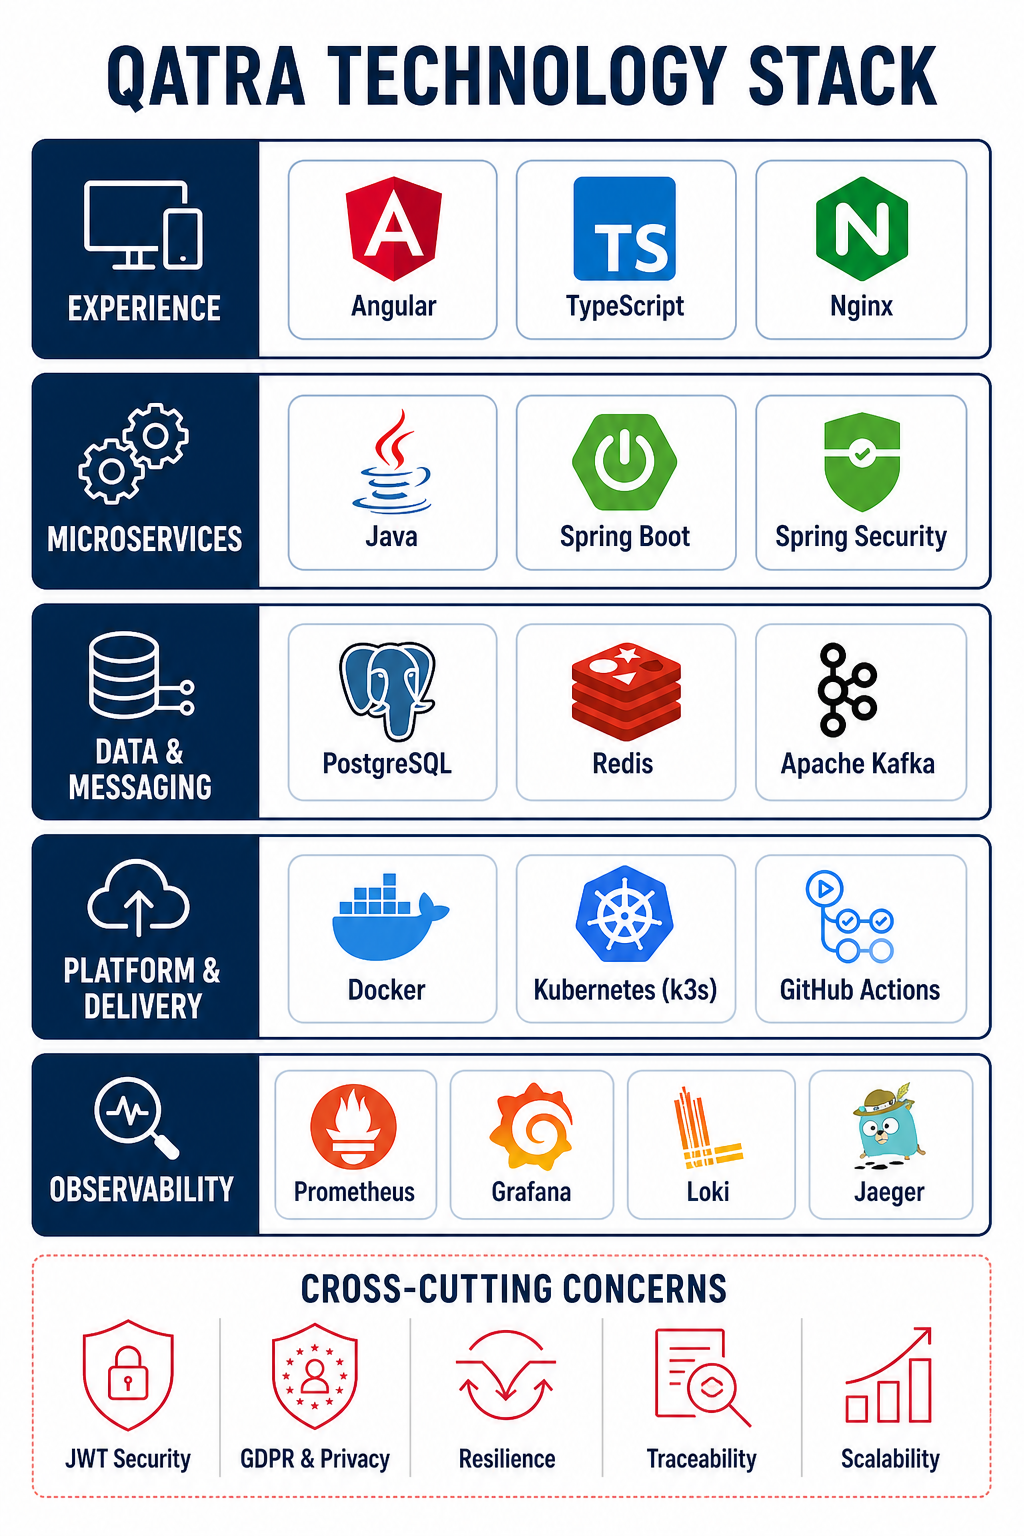
\includegraphics[width=0.82\textwidth,height=0.74\textheight,keepaspectratio]{assets/generated/technology-stack-portrait.png}
\caption{Qatra technology stack and engineering concerns}
\label{fig:technology-stack}
\end{figure}

\section{Development and Modeling Environment}
Table~\ref{tab:development-environment} lists tools verified from the supplied repositories and report workspace. It distinguishes artifacts that are present from tools that would merely be plausible for such a project.

\begin{table}[H]
\centering\small
\begin{tabularx}{\textwidth}{|P{3.2cm}|P{3.7cm}|Y|}
\hline
\rowcolor{tableheader}\textbf{Tool} & \textbf{Verified artifact} & \textbf{Role in the project}\\ \hline
Git and GitHub & Repository organization and GitHub Actions workflow files & Source-control workflow, pull-request CI, image publication, and deployment automation\\ \hline
StarUML & Supplied editable \texttt{.mdj} model & Requirements and global use-case modeling\\ \hline
Java 21 and Maven Wrapper & Service \texttt{pom.xml} files and wrapper scripts & Backend compilation, dependency management, and automated tests\\ \hline
Node.js and Angular CLI & \texttt{package.json}, lock file, and Angular workspace & Frontend development and production build orchestration\\ \hline
Docker and Docker Compose & Service Dockerfiles and root Compose file & Reproducible images and local multi-container integration\\ \hline
k3s and Traefik & Kubernetes manifests and \texttt{IngressRoute} resources & Server-side orchestration, routing, TLS entry, and operational services\\ \hline
PlantUML and \LaTeX & Editable diagram sources and report source & Reproducible UML figures and final academic documentation\\ \hline
\end{tabularx}
\caption{Verified development and modeling environment}
\label{tab:development-environment}
\end{table}

\section{Technology Decision Summary}
\begin{longtable}{|P{3.0cm}|P{3.5cm}|P{4.0cm}|P{3.2cm}|}
\hline
\rowcolor{tableheader}\textbf{Concern} & \textbf{Selected technology} & \textbf{Reason} & \textbf{Main caution}\\ \hline
Backend & Java 21, Spring Boot 4 & Typed domain model and integrated ecosystem & Framework and runtime complexity\\ \hline
Frontend & Angular 20 & Structured feature-rich SPA & Bundle size and test discipline\\ \hline
Persistence & PostgreSQL, JPA & Relational integrity and transactions & Query and migration governance\\ \hline
Events & Kafka & Decoupled notification processing & Eventual consistency and duplicates\\ \hline
Fast data & Redis & Low-latency operational state & Must not become undocumented authority\\ \hline
Packaging & Docker & Repeatable service images & Image and secret hygiene\\ \hline
Orchestration & k3s & Production-like Kubernetes model & Operational overhead\\ \hline
Delivery & GitHub Actions, GHCR & Repository-integrated automation & Secret and runner security\\ \hline
Metrics & Prometheus, Grafana & Time-series visibility and dashboards & Alert quality and retention\\ \hline
Logs/traces & Loki, Promtail, Jaeger & Cross-component diagnosis & Correlation and storage cost\\ \hline
\caption{Summary of selected technologies and trade-offs}
\label{tab:technology-summary}
\end{longtable}

\section*{Conclusion}
The selected stack is coherent with Qatra's functional scope and learning objectives. Its strength comes from the interaction between domain modularity, asynchronous communication, typed frontend integration, and operational visibility. The next chapter translates the project context into traceable requirements and a Kanban delivery model.
